\documentclass[uplatex,oneside]{jsbook}
\usepackage[deluxe,uplatex]{otf}
\usepackage[dvipdfmx]{color}
\usepackage[dvipdfmx]{graphicx}
\usepackage{framed}
\usepackage{wrapfig}
\definecolor{shadecolor}{gray}{0.9}
\definecolor{shadecolorb}{gray}{0.1}
\definecolor{reviewgreen}{rgb}{0,0.4,0}
\definecolor{reviewblue}{rgb}{0.2,0.2,0.4}
\definecolor{reviewred}{rgb}{0.7,0,0}
\definecolor{reviewdarkred}{rgb}{0.3,0,0}
\usepackage[utf8]{inputenc}
\usepackage{ascmac}
\usepackage{float}
\usepackage{alltt}
\usepackage{amsmath}

%% if you use @<u>{} (underline), use jumoline.sty
%%\usepackage{jumoline}

\newenvironment{shadedb}{%
  \def\FrameCommand{\fboxsep=\FrameSep \colorbox{shadecolorb}}%
  \MakeFramed {\FrameRestore}}%
 {\endMakeFramed}

\usepackage[top=10zw,bottom=12zw,left=10zw,right=10zw]{geometry}
%\usepackage[top=5zw,bottom=5zw,left=1zw,right=1zw]{geometry}

\newcommand{\parasep}{\vspace*{3zh}}
\setlength{\footskip}{30pt}

\usepackage[dvipdfmx,bookmarks=true,bookmarksnumbered=true,colorlinks=true,%
            pdftitle={Re:VIEWサンプル書籍},%
            pdfauthor={Re:VIEW Writers}]{hyperref}
% uplatexでのBookmarkの文字化け対策(日本語向け)
\usepackage[dvipdfmx]{pxjahyper}



\newenvironment{reviewimage}{%
  \begin{figure}[H]
    \begin{center}}{%
    \end{center}
  \end{figure}}

\newenvironment{reviewdummyimage}{%
  \begin{figure}[H]
    \begin{center}\begin{alltt}}{%
    \end{alltt}\end{center}
  \end{figure}}

\newenvironment{reviewemlist}{%
  \medskip\small\begin{shaded}\setlength{\baselineskip}{1.3zw}\begin{alltt}}{%
  \end{alltt}\end{shaded}}

\newenvironment{reviewlist}{%
  \begin{shaded}\small\setlength{\baselineskip}{1.3zw}\begin{alltt}}{%
  \end{alltt}\end{shaded}\par\vspace*{0.5zw}}

\newenvironment{reviewcmd}{%
  \color{white}\medskip\small\begin{shadedb}\setlength{\baselineskip}{1.3zw}\begin{alltt}}{%
  \end{alltt}\end{shadedb}}

\newenvironment{reviewbox}{%
  \medskip\small\begin{framed}\setlength{\baselineskip}{1.3zw}\begin{alltt}}{%
  \end{alltt}\end{framed}}

\newenvironment{reviewtable}[1]{%
  \begin{center}\small\setlength{\baselineskip}{1.2zw}
    \begin{tabular}{#1}}{%
    \end{tabular}
  \end{center}}

\newenvironment{reviewcolumn}{%
     \begin{framed}
  }{%
     \end{framed}
  \vspace{2zw}}

\newcommand{\reviewcolumnhead}[2]{%
{\noindent\large ■コラム: #2}}

\newcommand{\reviewtablecaption}[1]{%
  \caption{#1}}

\newcommand{\reviewimgtablecaption}[1]{%
  \caption{#1}\vspace{-3mm}}

\newcommand{\reviewbackslash}[0]{%
  \textbackslash{}}

\newcommand{\reviewlistcaption}[1]{%
  \medskip{\small\noindent #1}\vspace*{-1.3zw}}

\newcommand{\reviewemlistcaption}[1]{%
  \medskip{\small\noindent #1}\vspace*{-1.3zw}}

\newcommand{\reviewcmdcaption}[1]{%
  \medskip{\small\noindent #1}\vspace*{-1.3zw}}

\newcommand{\reviewindepimagecaption}[1]{%
  \begin{center}#1\end{center}}

\newcommand{\reviewboxcaption}[1]{%
  \medskip{\small\noindent #1}\vspace*{-1.3zw}}

\newcommand{\reviewimageref}[2]{図 #1}
\newcommand{\reviewtableref}[2]{表 #1}
\newcommand{\reviewlistref}[1]{リスト #1}
\newcommand{\reviewbibref}[2]{#1}
\newcommand{\reviewcolumnref}[2]{コラム #1}
\newcommand{\reviewsecref}[2]{#1}

\newcommand{\reviewminicolumntitle}[1]{%
  {\large ■メモ: #1}\\}


\newenvironment{reviewminicolumn}{%
  \vspace{1.5zw}\begin{screen}}{%
  \end{screen}\vspace{2zw}}

\newcommand{\reviewkw}[1]{\textbf{\textgt{#1}}}
\newcommand{\reviewami}[1]{\mask{#1}{A}}
\newcommand{\reviewem}[1]{\textbf{#1}}
\newcommand{\reviewstrong}[1]{\textbf{#1}}
\newcommand{\reviewunderline}{\Underline}

%% @<del> is ignored in LaTeX with default style
\newcommand{\reviewstrike}[1]{#1}

%%%% for ulem.sty:
%%\renewcommand{\reviewstrike}[1]{\sout{#1}}
%%
%%%% for jumoline.sty:
%%\renewcommand{\reviewstrike}[1]{\Middleline{#1}}

\newcommand{\reviewth}[1]{\textgt{#1}}
\newcommand{\reviewtitlefont}[0]{\usefont{T1}{phv}{b}{n}\gtfamily}
\newcommand{\reviewmainfont}[0]{}
\newcommand{\reviewcolophon}[0]{\clearpage}
\newcommand{\reviewappendix}[0]{\appendix}

\makeatletter
%% maxwidth is the original width if it is less than linewidth
%% otherwise use linewidth (to make sure the graphics do not exceed the margin)
\def\maxwidth{%
  \ifdim\Gin@nat@width>\linewidth
    \linewidth
  \else
    \Gin@nat@width
  \fi
}
\makeatother

\usepackage{reviewmacro}

\usepackage[T1]{fontenc}

\begin{document}

\reviewmainfont

\begin{titlepage}
  \begin{center}
    
\includegraphics[width=\textwidth,height=\textheight,keepaspectratio]{./images/cover.jpg}
  \end{center}
  \clearpage
\thispagestyle{empty}
\begin{center}%
  \mbox{} \vskip5zw
   \reviewtitlefont%
    {\Huge Re:VIEWサンプル書籍 \par}%
    \vskip 15em%
    {\huge
      \lineskip .75em
      \begin{tabular}[t]{c}%
        Re:VIEW Writers 著
      \end{tabular}\par}%
    \vfill
    {\large 2016-04-29 版\hspace{2zw} 発行\par}%
\vskip4zw\mbox{}
  \end{center}%
\end{titlepage}

\renewcommand{\chaptermark}[1]{{}}
\frontmatter

%%% originaltitle

%%% credit

%% preface
\chapter{はじめに}
\label{chap:preface}

(読者が読みたくなるようなまえがきっぽい言葉)

\section*{内容について}
\addcontentsline{toc}{section}{内容について}
\label{sec:-1}

(内容紹介)

\section*{動作環境について}
\addcontentsline{toc}{section}{動作環境について}
\label{sec:-2}

(バージョンとか)

\section*{謝辞}
\addcontentsline{toc}{section}{謝辞}
\label{sec:-3}

(必要に応じて)



\setcounter{tocdepth}{2}
\tableofcontents

\renewcommand{\chaptermark}[1]{\markboth{\prechaptername\thechapter\postchaptername~#1}{}}
\mainmatter
\chapter{サンプル}
\label{chap:ch01}

\begin{quotation}
書き方のサンプルです。上書きするなりして消して下さい。
\end{quotation}

\section{本文の書き方}
\label{sec:1-1}

最初の段落です。
この行も同じ段落です。

次の段落です。

2行以上以上空いていても1行空いているのと同様に処理します。

\subsection{見出し}
\label{sec:1-1-1}

「=」「==」「===」の後に一文字空白をあけると見出しになります。

\begin{reviewcolumn}
\hypertarget{column:ch01:1}{}
\reviewcolumnhead{}{コラムについて}

見出しの先頭に「[column]」と書くと、そこはコラムになります。

\end{reviewcolumn}

\section{箇条書き}
\label{sec:1-2}

番号のない箇条書きは「*」を使います。前後に空白を入れて下さい。

\begin{itemize}
\item 1つ目
\item 2つ目
\item 3つ目
\end{itemize}

番号つきの箇条書きには、「1.」「2.」などと書きます。
数字の値は実際には無視され、連番が振られます。

\begin{enumerate}
\item 1つ目
\item 2つ目
\item 3つ目
\end{enumerate}

\section{ソースコードなどのリスト}
\label{sec:1-3}

リストには「//list」ブロックや「//emlist」ブロックを使います。

\reviewlistcaption{リスト1.1: リストのサンプル}
\begin{reviewlist}
int main(int argc, char **argv) \{
  puts("OK");
  return 0;
\}
\end{reviewlist}

文中にリストを書くには「//emlist」になります。

\begin{reviewemlist}
def main
  puts "ok"
end
\end{reviewemlist}

\section{画像}
\label{sec:1-4}

画像は「//image」ブロックを使います。

\begin{reviewimage}
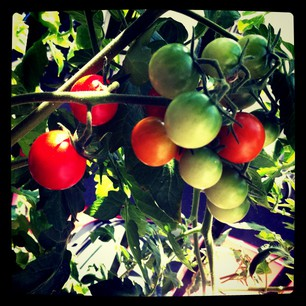
\includegraphics[width=\maxwidth]{./images/ch01-imgsample.jpg}
\caption{画像サンプル}
\label{image:ch01:imgsample}
\end{reviewimage}

より詳しくは、
\url{https://github.com/kmuto/review/blob/master/doc/format.rdoc}
を御覧ください。

\chapter{サンプルその2}
\label{chap:ch02}

基本はサンプルと同様です。


\renewcommand{\chaptermark}[1]{\markboth{\appendixname\thechapter~#1}{}}
\reviewappendix


%% backmatter begins
\backmatter



%%% profile

%%% advfile

%%% colophon
%% okuduke
\reviewcolophon
\thispagestyle{empty}

\vspace*{\fill}

{\noindent\reviewtitlefont\Large Re:VIEWサンプル書籍} \\
\rule[8pt]{14cm}{1pt} \\
{\noindent
2011年8月3日 v1.0.0版発行

\noindent
2016年4月29日 v2.0.0版発行
}

\begin{tabular}{ll}
著 者 & Re:VIEW Writers \\
編 集 & Re:VIEW Editors \\
発行所 & Re:VIEW Publishers \\

\end{tabular}
 \\
\rule[0pt]{14cm}{1pt} \\
(C) 2016 Re:VIEW Commiters \\

%%% backcover

\end{document}
